\begin{frame}
    \frametitle{\problemtitle}

    \begin{block}{Problem}
        Given a game of Wordle with a word of length $\ell$
        and $g$ guesses with $g-1$ guesses already made,
        find a valid final guess.
    \end{block}
    \pause

    \begin{block}{Observations}
        \begin{itemize}
            \item<+-> What can we learn from an existing guess?
            \begin{itemize}
                \item<+-> Green position: given letter is at that position.
                \item<+-> Yellow or gray position: given letter is not at that position.
                \item<+-> A letter appears in the solution at least as often as
                    the maximum number of green + yellow positions.
                \item<+-> If that letter also appears in a gray position, it
                    appears in the solution exactly as often as the maximum number of green + yellow positions.
            \end{itemize}
            \item<+-> So, for each letter, we have
            \begin{itemize}
                \item a list of positions in which it \emph{must} appear,
                \item a list of positions in which it \emph{must not} appear, and
                \item a lower and upper bound on the number of appearances.
            \end{itemize}
            \item<+-> How to find a word satisfying these requirements?
        \end{itemize}
    \end{block}
\end{frame}

\begin{frame}
    \frametitle{\problemtitle}

    \begin{block}{Observations}
        \begin{itemize}
            \item<1-> For each letter $\ell$, we have
            \begin{itemize}
                \item a list of positions in which it \emph{must} appear,
                \item a list of positions in which it \emph{must not} appear, and
                \item a lower bound $l_\ell$ and upper bound $u_\ell$ on the number of appearances.
            \end{itemize}
        \end{itemize}
    \end{block}

    \begin{block}{Solution}
        \vspace{1em}
        \begin{columns}
            \begin{column}[T]{0.6\textwidth}
                \begin{itemize}
                    \item<2-> First, consider simplified version where $l_\ell = 0$ for all $\ell$.
                    \item<3-> Solvable using max-flow
                    \begin{itemize}
                        \item Green positions: single incoming edge.
                        \item Otherwise: incoming edge for every possible character.
                    \end{itemize}
                \end{itemize}
            \end{column}

            \hfill

            \begin{column}[T]{0.25\textwidth}<3->
                \hspace*{-0.4\textwidth}% I have no clue what `columns` is trying to do here, but this fixes it XD
                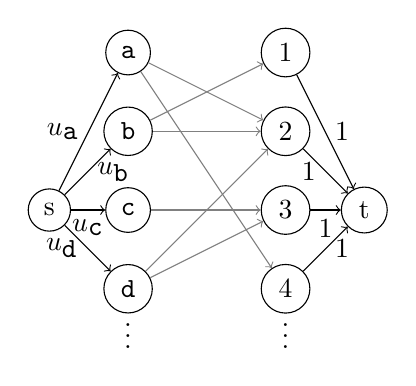
\begin{tikzpicture}
                    \node[circle,draw] (s) at (0, 0) {s};
                    \node[circle,draw] (a) at (1, 2) {\texttt{a}};
                    \node[circle,draw] (b) at (1, 1) {\texttt{b}};
                    \node[circle,draw] (c) at (1, 0) {\texttt{c}};
                    \node[circle,draw] (d) at (1, -1) {\texttt{d}};
                    \node[draw=none] at (1, -1.5) {$\vdots$};
                    \draw[->] (s) -- (a) node[midway,anchor=east] {$u_{\text{\texttt{a}}}$};
                    \draw[->] (s) -- (b) node[midway,anchor=west] {$u_{\text{\texttt{b}}}$};
                    \draw[->] (s) -- (c) node[midway,anchor=north] {$u_{\text{\texttt{c}}}$};
                    \draw[->] (s) -- (d) node[midway,anchor=east] {$u_{\text{\texttt{d}}}$};
                    \node[circle,draw] (p1) at (3, 2) {1};
                    \node[circle,draw] (p2) at (3, 1) {2};
                    \node[circle,draw] (p3) at (3, 0) {3};
                    \node[circle,draw] (p4) at (3, -1) {4};
                    \node[draw=none] at (3, -1.5) {$\vdots$};
                    \node[circle,draw] (t) at (4, 0) {t};
                    \draw[->] (p1) -- (t) node[midway,anchor=west] {1};
                    \draw[->] (p2) -- (t) node[midway,anchor=east] {1};
                    \draw[->] (p3) -- (t) node[midway,anchor=north] {1};
                    \draw[->] (p4) -- (t) node[midway,anchor=west] {1};
                    \draw[->,color=gray] (b) -- (p1);
                    \draw[->,color=gray] (a) -- (p2);
                    \draw[->,color=gray] (b) -- (p2);
                    \draw[->,color=gray] (d) -- (p2);
                    \draw[->,color=gray] (c) -- (p3);
                    \draw[->,color=gray] (d) -- (p3);
                    \draw[->,color=gray] (a) -- (p4);
                \end{tikzpicture}
            \end{column}
        \end{columns}
    \end{block}
\end{frame}

\begin{frame}
    \frametitle{\problemtitle}

    \begin{block}{Solution}
        \vspace{1em}
        \begin{columns}
            \begin{column}[T]{0.4\textwidth}
                \begin{itemize}
                    \item<1-> Multiple ways to extend this to arbitrary lower bounds.
                    \begin{itemize}
                        \item<2-> If you have the code: min-cost max-flow.
                    \end{itemize}
                    \item<3-> Also possible: more clever max-flow modelling.
                    \begin{itemize}
                        \item Edge from $s$ to a letter $\ell$ has capacity $l_\ell$;
                        \item Edge from  $s'$ to a letter $\ell$ has capacity $u_\ell - l_{\ell}$.
                    \end{itemize}
                \end{itemize}
            \end{column}

            \hfill

            \begin{column}[T]{0.5\textwidth}<3->
                \hspace*{-0.2\textwidth}% I have no clue what `columns` is trying to do here, but this fixes it XD
                % WIP
                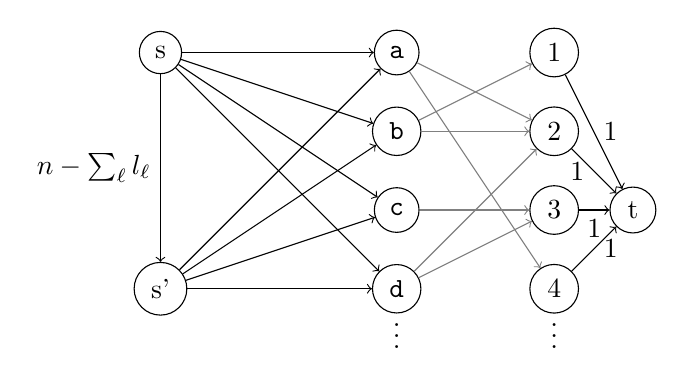
\begin{tikzpicture}
                    \node[circle,draw] (s) at (-2, 2) {s};
                    \node[circle,draw] (sp) at (-2, -1) {s'};
                    \node[circle,draw] (a) at (1, 2) {\texttt{a}};
                    \node[circle,draw] (b) at (1, 1) {\texttt{b}};
                    \node[circle,draw] (c) at (1, 0) {\texttt{c}};
                    \node[circle,draw] (d) at (1, -1) {\texttt{d}};
                    \node[draw=none] at (1, -1.5) {$\vdots$};
                    \draw[->] (s) -- (a);% node[midway,anchor=south east] {$l_{\text{\texttt{a}}}$};
                    \draw[->] (s) -- (b);% node[midway,anchor=south] {$l_{\text{\texttt{b}}}$};
                    \draw[->] (s) -- (c);% node[midway,anchor=west] {$l_{\text{\texttt{c}}}$};
                    \draw[->] (s) -- (d);% node[midway,anchor=north] {$l_{\text{\texttt{d}}}$};
                    \draw[->] (sp) -- (a);% node[midway,anchor=south east] {$u_{\text{\texttt{a}}} - l_{\text{\texttt{a}}}$};
                    \draw[->] (sp) -- (b);% node[midway,anchor=south] {$l_{\text{\texttt{b}}}$};
                    \draw[->] (sp) -- (c);% node[midway,anchor=west] {$l_{\text{\texttt{c}}}$};
                    \draw[->] (sp) -- (d);% node[midway,anchor=north] {$l_{\text{\texttt{d}}}$};
                    \draw[->] (s) -- (sp) node[midway, anchor=east] {$n - \sum_{\ell} l_{\ell}$};
                    \node[circle,draw] (p1) at (3, 2) {1};
                    \node[circle,draw] (p2) at (3, 1) {2};
                    \node[circle,draw] (p3) at (3, 0) {3};
                    \node[circle,draw] (p4) at (3, -1) {4};
                    \node[draw=none] at (3, -1.5) {$\vdots$};
                    \node[circle,draw] (t) at (4, 0) {t};
                    \draw[->] (p1) -- (t) node[midway,anchor=west] {1};
                    \draw[->] (p2) -- (t) node[midway,anchor=east] {1};
                    \draw[->] (p3) -- (t) node[midway,anchor=north] {1};
                    \draw[->] (p4) -- (t) node[midway,anchor=west] {1};
                    \draw[->,color=gray] (b) -- (p1);
                    \draw[->,color=gray] (a) -- (p2);
                    \draw[->,color=gray] (b) -- (p2);
                    \draw[->,color=gray] (d) -- (p2);
                    \draw[->,color=gray] (c) -- (p3);
                    \draw[->,color=gray] (d) -- (p3);
                    \draw[->,color=gray] (a) -- (p4);
                \end{tikzpicture}
            \end{column}
        \end{columns}
    \end{block}

    \only<4->{
        \solvestats
    }
\end{frame}
